\chapter{Review of Related Literature}
\section{Artificial Intelligence in Imperfect Information Games}
Games can be classified as an imperfect information game by having incomplete information about the current game state for both players \cite{StudeGame, 2509_03682v1}. An example would be in MOBAs (Multiplayer Online Battle Arena), the fog of war mechanic hides portions of the map, including objectives and enemy positions, from both teams. By placing a tool, such as a ward in League of Legends or an observer in Dota 2, the player gains a temporary vision in the map for strategic planning \cite{WARDS}. This feature engages players to create strategic reasoning under certainty, utilizing prediction, coordination, and resource management to gain informational advantages over opponents. Games have a history of being a metric on how AI progresses and performance in the current time \cite{StudeGame, GamePer}. The case is the same for both perfect information and imperfect information games \cite{StudeGame}. For perfect information games, like chess, they primarily use Alpha-Beta pruning, a search algorithm that uses trees to explore possible chess moves and prunes the branches that will not affect the final decision \cite{alphabeta}. In imperfect information games, a search algorithm like Alpha-Beta Pruning would be difficult to implement because the algorithm is made for perfect information games \cite{alphabe}. A popular algorithm that is used in imperfect information games would be Monte Carlo Tree Search with Reinforcement Learning because MCTS has integration with neural network systems like AlphaZero \cite{AIAgent, AlphaStratego}. In terms of reinforcement learning, the training focuses on trial and error to provide the best possible decision \cite{comprel}. Continuing development of AI algorithms in imperfect information games advances our understanding of decision-making under uncertainty and promotes strategic planning.


\subsection{Student of Games}
A unified learning algorithm that can support both perfect information and imperfect information is Student of Games. Combining self-play learning, strategic search, and principles from game theory \cite{StudeGame}. SoG achieved strong performance in Chess and Go in perfect information games and in imperfect information games like heads-up no-limit Texas hold ’em poker, and defeated the state-of-the-art agent in Scotland Yard. When comparing to MARL, SoG supports and has been tested in both game types and uses game theoretic reasoning, which computes or approximates the Nash equilibria. MARL with DQN uses trial and error learning and self-play learning, which relies on the exploration of the environment. MARL has also been tested in complex video games \cite{2509_03682v1}, unlike SoG, which has not been tested in video games.

\subsection{Deep Q-Networks and Dueling Architectures}
Deep Q-networks (DQN) and their variants have become a standard framework for decision-making in complex environments with high-dimensional observations. Hessel et al. (2021) combined several independent improvements to DQN—such as double Q-learning, prioritized replay, dueling networks, and noisy nets—into a unified agent called Rainbow, demonstrating state-of-the-art performance on competitive benchmarks \cite{RainbowJMLR2021}. This demonstrates that carefully integrating architectural and algorithmic improvements can substantially improve both data efficiency and final performance in value-based deep RL.

A key architectural component of Rainbow is the dueling network architecture, proposed by Wang et al. (2016) and detailed in modern surveys \cite{RainbowJMLR2021, DRLImperfectInfo2023}. This design splits the Q-function into a state-value stream and an advantage stream. This split allows the network to generalize across actions and improves policy evaluation, particularly in environments with many similar-valued actions. Our MARQ model builds on this idea by feeding the shared ResNet-based representation into dueling value and advantage streams, which is particularly beneficial in board games where many positions have similar strategic value.


\subsection{Multi-Agent Reinforcement Learning}
Reinforcement Learning can solve complex problems through trial and error, by learning from the environment to be able to provide optimal decisions \cite{2509_03682v1}. This can be the case for Single-Agent Reinforcement Learning(SARL). SARL has its limits in solving many real-world problems. Multi-Agent Reinforcement Learning(MARL) was introduced as a solution for the challenges of SARL, by having multiple agents in an environment that interact with each other, the decisions they could make would be optimized \cite{2509_03682v1}. Optimized, meaning that these agents go through trial and error together to make the best decision given the reward. As for the implementation of this in Stratego, two agents would compete with each other to know the optimal decisions given the environment, which has imperfect information and opposing strategies.
As MARL has its advantages, it also has challenges. The first would be Non-Stationarity, and the second is scalability, as for non-stationarity, each agent learns simultaneously, meaning the environment constantly changes \cite{MARLCHALL}. For scalability, as more agents are being used, the computational power rises, making it expensive \cite{CFRMIX, MARLCHALL}. Recent work on Ataraxos demonstrates that these challenges can be addressed through careful regularization: by constraining policy updates toward both exploratory (uniform) and stable (target network) anchors with time-varying coefficients, agents can achieve superhuman performance in complex imperfect-information games while maintaining training stability \cite{Ataraxos2025}.


\subsection{Counterfactual Regret Minimization}
Counterfactual Regret Minimization(CFR) is an iterative algorithm that approximates the Nash equilibria commonly used on imperfect information games like poker and Stratego \cite{CFRMIX,xu2024dynamic}. The Nash equilibria are what CFR approximates to make the best possible decision with minimal regret. Regret in this scenario is the what-ifs of the algorithm if the algorithm chooses the other decision. For CFR to make decisions, it repeatedly minimizes regret to approximate the Nash equilibria \cite{CFRMIX}. Other works have made variations of the base CFR, showing improved convergence rate, but require a significant amount of effort by researchers. A framework is proposed named AutoCFR, instead of relying on manually crafted algorithms, it automatically designs new CFR variants using an outer loop to search over algorithm designs and an inner loop to test them on equilibrium finding tasks \cite{xu2022autocfr}. 

\subsection{Opponent Modeling in Imperfect-Information Games}
In imperfect-information games, an agent’s optimal strategy depends not only on the environment but also on the behavior of the opponent. Classical opponent modeling often builds models from observed action frequencies, and computes best responses in a game-theoretic framework. Li et al. (2024) formalize opponent-model search in games with incomplete information, providing algorithms to compute optimal or robust strategies given various forms of opponent knowledge \cite{li2024opponent}.

In the deep RL setting, modern approaches encode observations of opponents directly into the network trunk, jointly learning a policy and an opponent model without explicitly predicting actions \cite{DRLImperfectInfo2023}. This shows that learning implicit opponent representations from interaction traces can be more effective than handcrafted models, especially in high-dimensional state spaces. Our AAREN module follows this tradition of implicit opponent modeling but is specialized to board games with hidden piece identities. Instead of maintaining explicit probability distributions over opponent piece types, AAREN aggregates observed opponent action sequences into dense embedding vectors. These vectors are then concatenated as additional input channels to the Q-network, allowing the agent to reason about the opponent’s likely pieces and strategy in a learned representation space.




\section{RNN}
Recurrent Neural Network is a type of Neural Network designed to process sequential data. Unlike common Neural Networks, RNNs have a memory because the information passed to the next step is based on the memory from the previous step. RNN can be applied to imperfect information games such as Stratego because of its memory. By using the memory to remember the pieces that have been revealed, the decision could be optimized \cite{AIAgent}.

\subsection{History Aggregation and State Representation Learning}
Learning from histories is a central challenge in partially observable and non-Markovian environments. Wang et al. (2026) show how to systematically construct non-Markovian decision processes by aggregating interaction histories into state representations, providing an effective way to add temporal dependencies into RL \cite{wang2026history}. By explicitly modeling history via learned aggregators, an agent can better handle complex temporal structures.

More broadly, representation learning for RL has explored the use of embeddings to generalize across states and goals. Echchahed and Castro (2025) highlight in their survey that separating dynamics from rewards allows policies to be transferred across tasks through learned representations \cite{echchahed2025srl}. Our AAREN embeddings can be viewed as a form of history-dependent state representation that encodes the opponent’s action history into a compact vector to augment the board state. This approach is tailored to the specific structure of imperfect-information board games where opponent behavior reveals hidden state. By learning these embeddings jointly with the Q-network, we avoid the need to handcraft belief distributions and instead let the network infer implicit piece identities from observed behavior.
\subsection{LSTM}
Long Short-Term Memory is a popular RNN variant that has the capabilities of RNN but also processes data with long-term dependencies \cite{ALSELWI2024102068}. LSTM mitigates the vanishing gradient problem that RNN faces. The vanishing gradient problem is basically as in the name, vanishing gradient, as color in a gradient, the message in this case starts strong and gradually fades away when it passes through each layer, making the learning weak or close to zero. LSTM can be used to solve imperfect information games because of its capability to process data with long-term dependencies while having the memory of RNN.
\subsection{Aaren}
Aaren, known as Attention as a recurrent neural network, combines the parallel training efficiency of Transformers with the streaming update efficiency of RNNs \cite{Aaren}. Aaren, like transformers, can be trained in parallel as well as RNN, can process sequential data with memory. In the study, Aaren was tested in event forecasting, time series forecasting, and classifications. Aaren achieved similar accuracy to Transformers but was more time and memory-efficient.

\subsection{Residual Networks and Self-Attention in Board Games}
Residual networks (ResNets) have become a common backbone in modern board-game RL systems. AlphaZero-style agents for Go, chess, and Stratego use a deep tower of residual convolutional blocks as the network trunk, enabling stable training of deep networks that can capture spatial dependencies on the board \cite{AlphaStratego}. Modern architectures often mix these residual blocks with self-attention layers to bridge local and global knowledge. This hybrid architecture significantly improves playing strength in board games by better handling long-range patterns \cite{restnet2025board}.

Because of these results, our architecture adopts a ResNet backbone with spatial self-attention. This allow each board position to attend to all other positions, capturing long-range piece relationships that are difficult to represent with purely convolutional architectures. We extend this line of work by combining self-attention with a dueling Q-network and a learned opponent embedding, addressing the additional challenges of imperfect information and opponent modeling in Stratego.


\section{Stratego}
The origin of Stratego can be traced to a traditional board game called Jungle, where instead of human pieces instead it used animals. In the jungle, the pieces are not hidden, making it a perfect information game. Stratego is a two-player board game where players each have a 40-piece army. In the tabletop version of Stratego, one player is assigned to the blue army and the other player is assigned to the red army. Each army has a flag assigned to it, which cannot be moved when the game starts. There are a total of 80 troop pieces, while the total number of variations is 12. The pieces rank range from 1 to 10, and a piece that's not numbered is a bomb and the flag. The player also has time to move pieces before the game starts to make use of the fog of war and create creativity and optimal positions on the board. As the pieces have ranks, the higher the number, the higher the power. There is an instance where the lower-ranked can defeat a higher-ranked ranked, which is the piece that has a rank of one, named the spy, can defeat the strongest piece that has a rank of ten, named the marshal, if the spy attacks first. As for the bombs, almost all pieces are vulnerable except the miner, the only one who can defuse the bomb. And the pieces that cannot be moved are the bomb and the flag. Another piece that has a special ability is the scout; it can move either horizontally or vertically, not just one square. If both pieces have the same number, and the piece attacks, both of them would be eliminated. There are multiple win conditions in Stratego. The obvious one would be capturing the flag, another one would be that the opponents have no mobile pieces, another would be that there are no miners that can defuse the bomb to capture the flag, and lastly, the opposing player had the time run out.

\subsection{Deep Reinforcement Learning in Stratego}
Stratego is a popular imperfect-information board game where players must reason about hidden piece identities over long time horizons. Pérolat et al. (2022) demonstrated with DeepNash that a model-free multiagent RL approach can reach human expert level in Stratego, using deep convolutional networks trained with game-theoretic regularization \cite{perolat2022stratego}. Their architecture relies heavily on ResNet-style networks to process board features under imperfect information. More recent work has further improved these baselines by combining self-play reinforcement learning with test-time search, achieving superhuman performance \cite{Ataraxos2025}.

Our MARQ framework is closely related to these systems in its use of a deep ResNet backbone, but we explicitly incorporate opponent modeling via AAREN embeddings. By basing the agent on the opponent’s observed actions, we allow the agent to adapt to specific opponents and exploit behavioral patterns. This adds to the equilibrium-style play of prior models with learned opponent representations.

\begin{figure}[h]
    \centering
    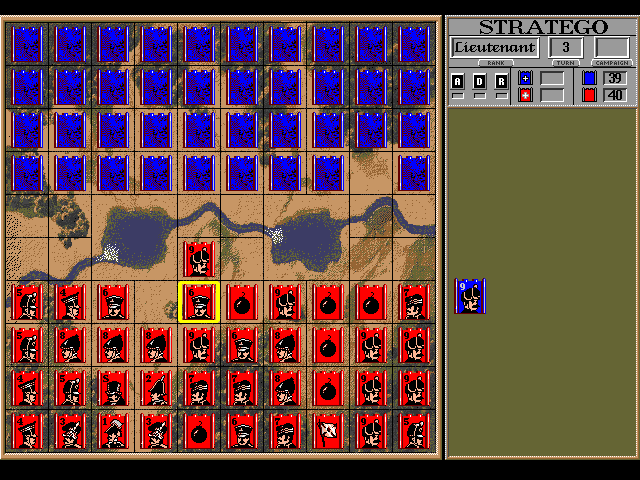
\includegraphics[width=0.7\textwidth]{figures/stratego.png}
    \caption{Stratego Game board.}
    \label{fig:stratego_review}
\end{figure}



\section{Board Games in Community Building}
Modern board games are becoming more widespread, expanding their market share each year. During COVID-19 lockdowns, board game sales increased because people were stuck at home with family and had free time. Also, playing board games during that time helped with stress, isolation, and anxiety. Certain games like Pandemic, a cooperative strategy board game where players work together to stop global disease outbreaks by discovering cures before time runs out, became more popular due to their reflection of the real-world scenario. Board game communities differ between the West and the East \cite{boardgamehk}. From the east, board games are considered social activities, while in the west, board games grew as hobbies, communities focusing on the gameplay and mechanics. In Hong Kong, there are two distinct board game communities named BGHK and Oasis. BGHK consists of Cantonese-speaking individuals who treat board games as social bonding. They even event sessions for "party game days" and "welcome newbies," emphasizing making friends rather than the game itself. While the Oasis group focuses on the hobby, playing newly released and complex games. Attracting players with the mechanics and novelty rather than just socializing. A study has been made to use board games as an answer to the problem of difficulty in creating a sense of "togetherness or kinship," and board games have advantages for improving the cognitive function of older people \cite{Boardgames}. In the study, the Tresna Werdha Budi Pertiwi Social Home has a problem of having a sense of family among residents. By playing together, the elderly had consistent interaction with each other, reducing the feeling of loneliness and detachment. Board games not only provide entertainment but also memory stimulation and improve social bonds. Board games provide a face-to-face interaction requiring people to sit together at a table, unlike in video games, where players are often separate from each other \cite{boardgamecom}. Every shared experience creates a unique microenvironment where players enter a separate reality governed by the game's rules. In the space, the players share emotions and strategy. Sharing these emotions helps strengthen friendships, family bonds, and trust. Many board game players first connect through gaming with friends and family, which can branch out to dedicated groups or conventions, and expand their social circle.

\section{Other Applications}
An extension of MARL with DQN was demonstrated in robotics. In these environments, robots are trained to make decisions based on rewards. The study assigned different energy costs to each robotic arm, allowing the robot to learn how to adjust its movement based on cost, using less energy when the reward is small and exerting more effort if the reward is appropriate \cite{robotmarl}. MARL with Deep Q-learning was also used in traffic signal control. Applied a cooperative multi-agent DQN framework to manage six interconnected intersections, where each intersection acted as an independent learning agent. Using the SUMO simulator, each agent selected signal phases to minimize congestion and improve overall traffic flow. Their approach introduced a reward function based on the standard deviation of stopping vehicles across lanes, showing balanced lane utilization rather than simply reducing queue lengths. This design showed that MARL with DQN can enhance not only traffic efficiency but also environmental sustainability by reducing emissions and fuel consumption. In businesses in developing countries, it is essential that growth should be the top priority; however, this creates a problem in increasing taxation for improving infrastructure to further support the current population. Using MARL, we can create a model system where multi-agent RL acts as different parties that discover the optimal tax policies without needing to rely on traditional economic models \cite{MARLEcon}.

\section{Application to Other Game Environments}
Although this study focuses on Stratego as the game environment, the MARQ framework can also be applied to other strategic and simulation-based games that involve decision-making and hidden information. Sports management titles such as Madden NFL's Dynasty Mode, NBA 2K's franchise mode, Esports Manager, and Football Manager feature complex systems of player development, transfer, and long-term planning, where agents must act without complete information about the future player performance and market behavior. In these environments, the MARQ framework could model AI agents capable of learning optimal trade strategies or budget allocations through reinforcement learning. The framework's belief-state modeling would allow the AI to check hidden player attributes or opponent strategies, while the Deep Q-Network could optimize sequential decisions across multiple simulated seasons.

Similarly, the framework could be applied to a game called Clash Royale, where players must make fast tactical decisions without full knowledge of their opponent's hand or resource level. The Probabilistic Belief State in this setting could estimate the likelihood of specific opponent cards being available, while the Deep Q-Network would select optimal actions for troop deployment and timing. IS-MCTS could be used to search over possible opponent hands, enabling informed decision-making for lane control or counter-attack scenarios.


